This Online Appendix expands on some of the analyses presented in the main body of the paper. First, it characterizes the treated municipalities in our analytical samples relative to the average Chilean municipality. Second, it shows the effects of \emph{Plan Cuadrante} on different types of crime. Third, it documents some differences in results associated to private investment in security depending on household SES. Fourth, it presents two new analyses that suggest that changes in police resources associated to the adoption of the \emph{Plan Cuadrante} are not enough to explain its results. Fifth, it examines what factors are associated with a larger increase in police resources across municipalities adopting \emph{Plan Cuadrante}. Sixth, it presents the results of a new exercise that shows that increases in police resources unrelated to \emph{Plan Cuadrante} do not generate major gains in police effectiveness. Finally, it shows that the comparison of perceived police performance between early and late adopters is not confounded by differences in adoption timing.


\subsection{Characterization of the Analytical Samples}
\label{sec:ext_validity}

The treated municipalities in our analytical samples are geographically distributed across the country. As shown in Figure \ref{fig:pcsp_maps}, the 46 treated municipalities in the ENUSC-based sample span Chile from north to south, covering a wide range of geographic and socioeconomic contexts, and together account for approximately 27\% of Chile's population. The 96 treated municipalities in the administrative data sample provide even broader national coverage, together accounting for over half of Chile's population.

Table \ref{tab:comparing_samples} characterizes the treated municipalities in each analytical sample relative to all Chilean municipalities (Column 1), all \emph{Plan Cuadrante} municipalities (Column 2), the always-treated municipalities excluded from our estimation samples (Column 3), and never-treated municipalities (Column 6). Columns (4) and (5) report characteristics for the treated municipalities in the ENUSC and administrative data analytical samples respectively. On several dimensions our samples broadly resemble the overall Chilean population: the poverty rate of the 46 treated municipalities in the ENUSC sample (21.7\%) and the 96 treated municipalities in the administrative data sample (24.0\%) are both close to the national average of 23.7\%, and the crime rates of the treated ENUSC municipalities closely track the average across all \emph{Plan Cuadrante} municipalities (2,202 vs.\ 2,132 per 100,000 inhabitants). They do differ on other dimensions---particularly crime rates relative to all Chilean municipalities and population density---but both differences have natural explanations. Higher crime rates are expected because \emph{Plan Cuadrante} exclusively targeted urban municipalities, where crime is more prevalent. The lower-than-average population density in our samples (215 and 135 inhabitants per km$^2$, vs.\ a national mean of 870) reflects the fact that the most densely populated \emph{Plan Cuadrante} municipalities---those of the Santiago metropolitan area---were the earliest adopters of the program and are therefore excluded from our analytical samples as always-treated. 

\begin{figure}[h!]
    \centering
    \caption{Geographic Distribution of \emph{Plan Cuadrante}}
    \label{fig:pcsp_maps}
    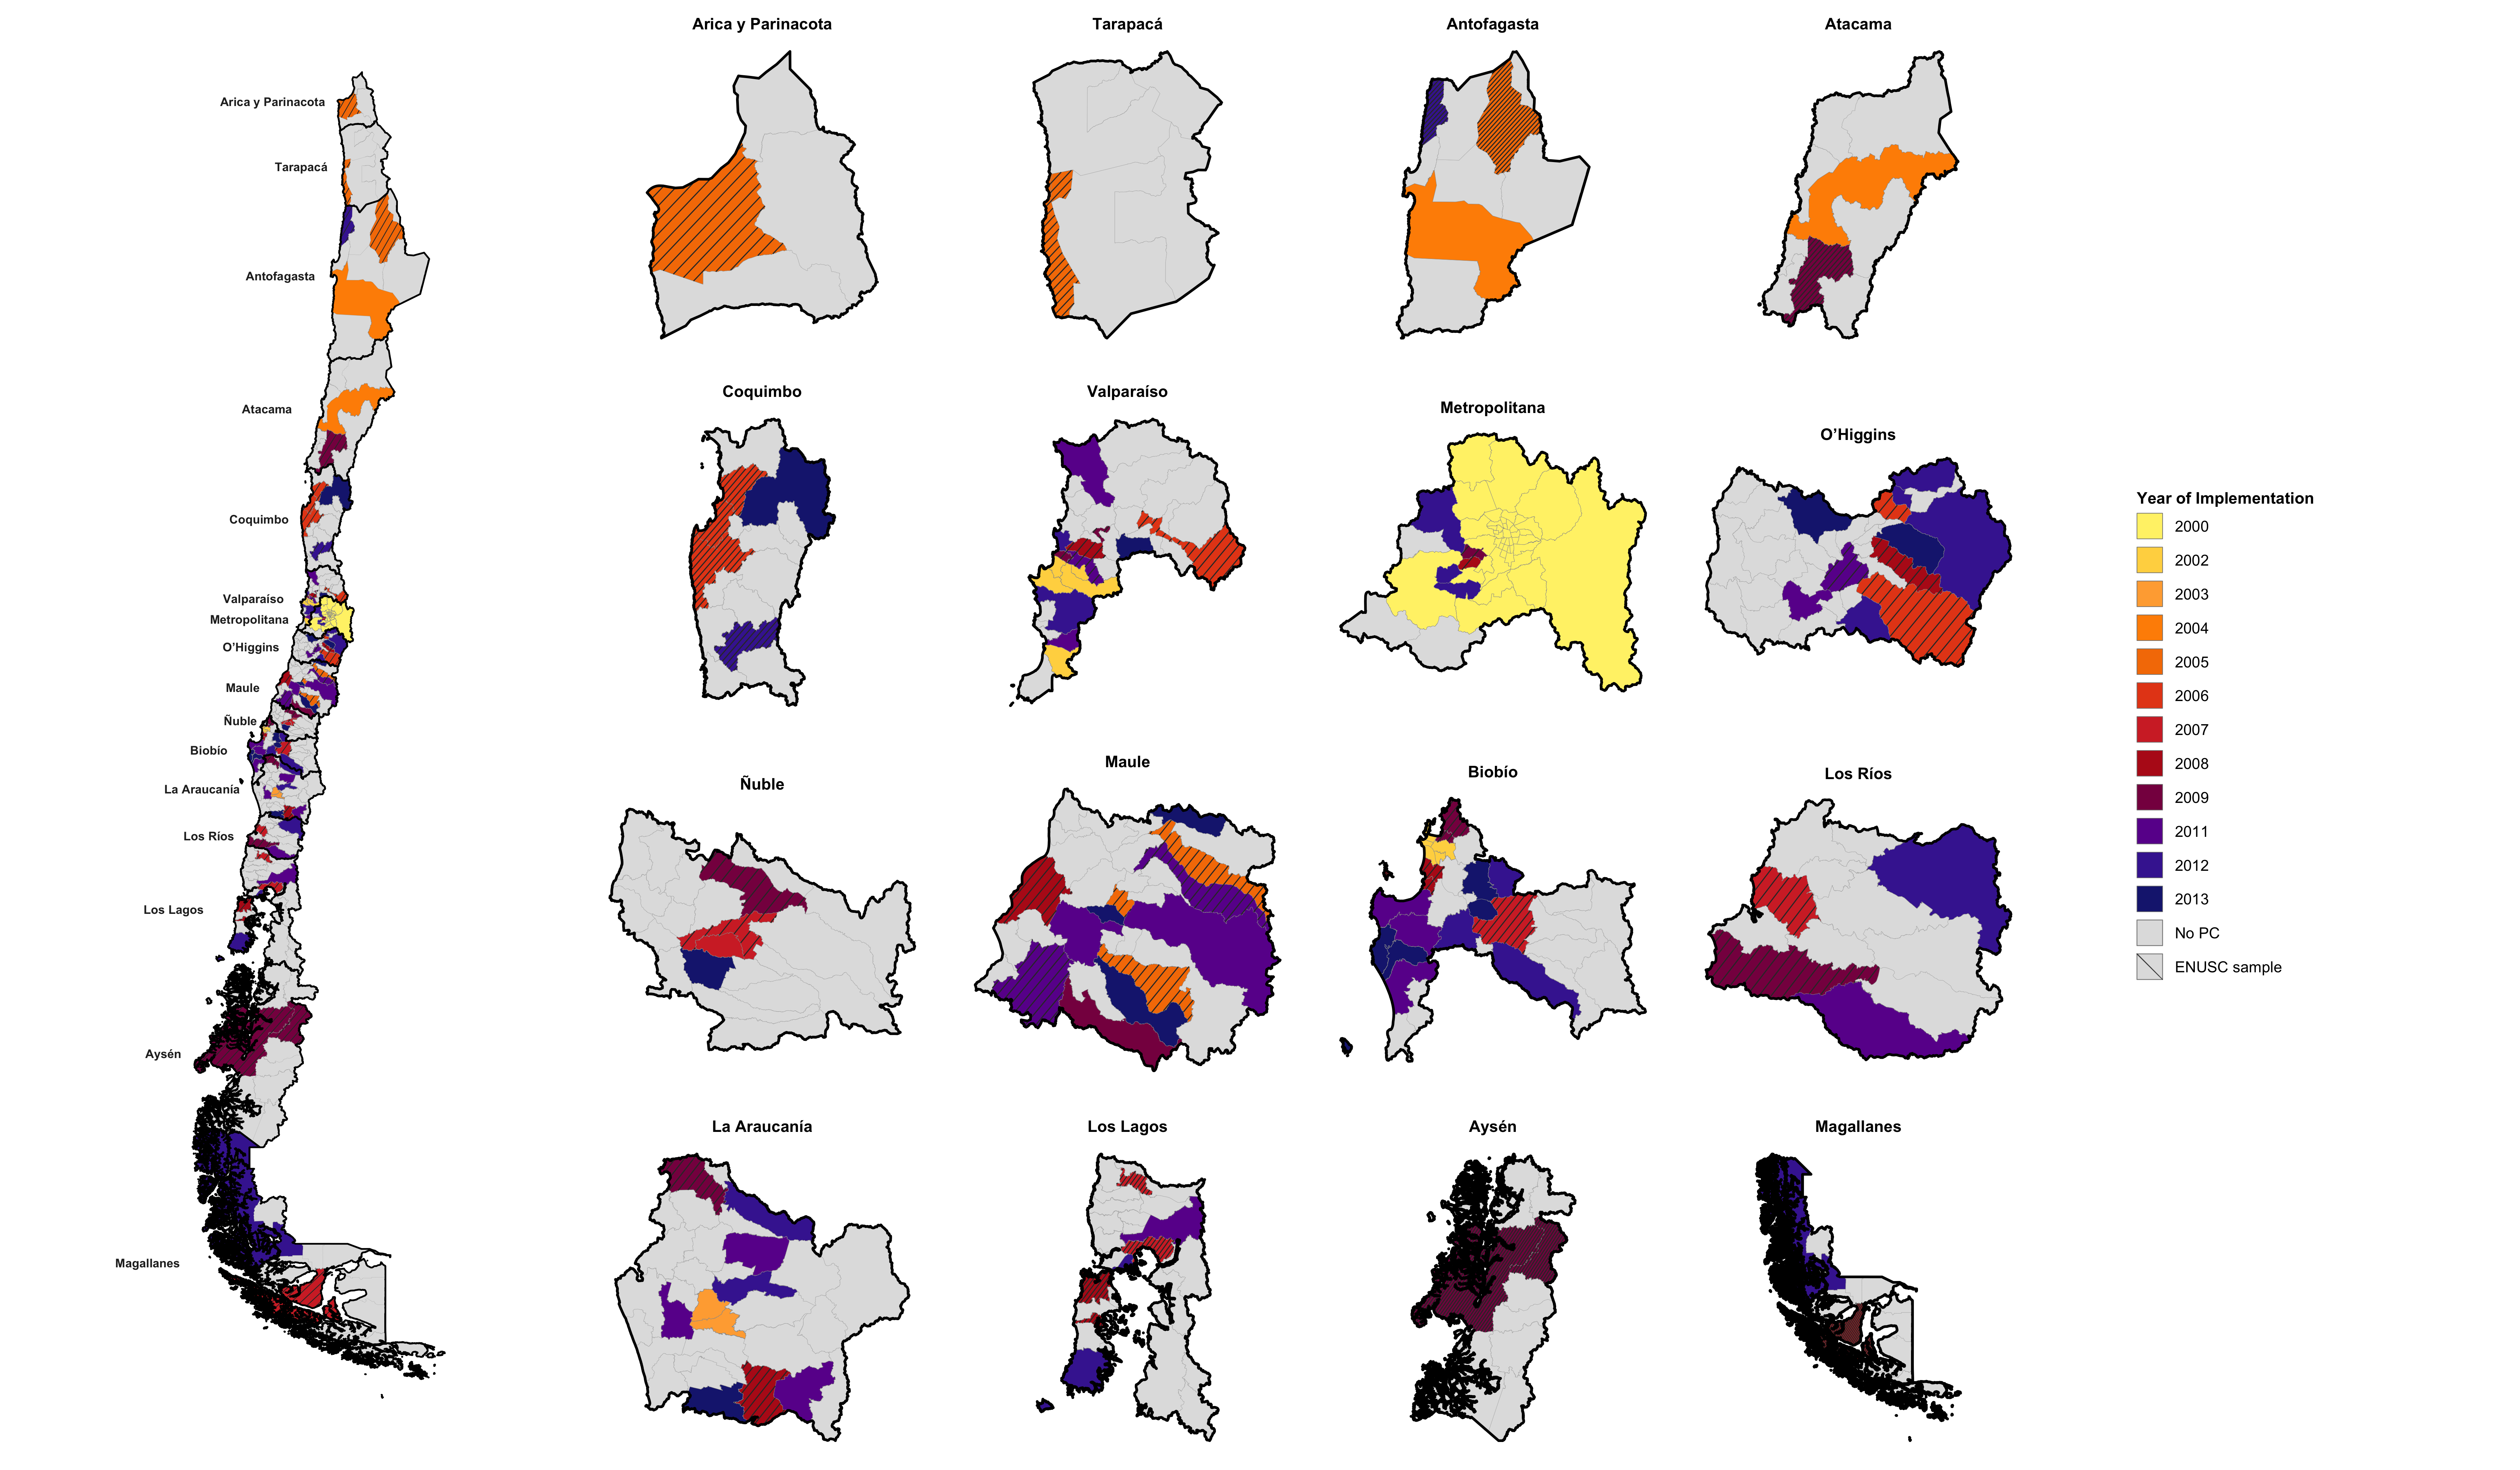
\includegraphics[width=\textwidth]{../manuscript/Graphs/mapa_PCSP_Chile_combinado.png}
    \begin{minipage}{0.95\textwidth}
    \footnotesize
    Notes: This figure shows the spatial rollout of \emph{Plan Cuadrante} across Chilean municipalities. The national map (left) is displayed alongside the 16 regional maps (right) for closer inspection. The color of each treated municipality indicates its year of program adoption, ranging from 2000 (lightest) to 2013 (darkest), following the legend. Municipalities shown in light grey were never treated under PC. Diagonal hatching identifies the 46 treated municipalities in the analytical sample used to estimate the effects on ENUSC outcomes.
    \end{minipage}
\end{figure}


\begin{table}[H]
\caption{Baseline characteristics by subsample}
\label{tab:comparing_samples}
\begin{center}
\resizebox{\textwidth}{!}{
\begin{threeparttable}
\begin{tabular}{l cccccc}
\toprule
&  & \multicolumn{4}{c}{PC municipalities}  & \\
\cmidrule(lr){3-6}
& (1) & (2) & (3) & (4) & (5) & (6) \\
& All & All PC & Always- & Treated & Treated & Never- \\
& municipalities & municipalities & treated & ENUSC & admin.\ data & treated \\
\midrule
Reported crime (per 100k pop.) &     1,650.23 &     2,132.29 &     2,437.25 &     2,202.06 &     1,976.59 &     1,282.47 \\
Arrests (per 100k pop.)        &       267.62     &       442.08     &       606.01     &       459.05     &       358.11     &       134.11     \\
Poverty rate (\%)              &        23.73     &        20.50     &        14.88     &        21.73     &        23.96     &        26.82     \\
Pop.\ density (pop./km$^2$)   &       870.28 &     1,904.14 &     4,593.32 &       215.52 &       134.50 &        27.02 \\
Population                     &    57,857.22         &   117,975.43         &   187,558.74         &   113,079.74         &    81,532.84         &    11,612.44         \\
\midrule
Municipalities                 &          346            &          150            &           58            &           46            &           96            &          196            \\
\bottomrule
\end{tabular}
\begin{tablenotes}[flushleft]
\footnotesize{\item Note: Reported crime, poverty rate, population density, and population are measured as of 2003; arrests are measured as of 2005, the first year for which arrest data are available. Column (1) includes all municipalities in Chile. Column (2) includes all PC municipalities. Column (3) restricts to municipalities that adopted \emph{Plan Cuadrante} before 2005, the always-treated in our sample, which are therefore excluded from our estimation samples (as depicted in Figure 1, panel (a)). Column (4) restricts to treated municipalities in the analytical sample using the ENUSC data. Column (5) restricts to treated municipalities included in the analytical sample using the administrative data. Column (6) includes never-treated municipalities.}
\end{tablenotes}
\end{threeparttable}}
\end{center}
\end{table}


\clearpage

\subsection{Effects of \emph{Plan Cuadrante} on Different Types of Crime}
Figure \ref{fig:figureA8} displays the effects of \emph{Plan Cuadrante} on victimization by type of crime, showing beneficial effects for both violent and property crimes. 


\begin{figure}[h!]
    \centering
    \caption{The Effects of \emph{Plan Cuadrante} on Victimization and Reported Crime by Type of Crime}
    \label{fig:figureA8}
    \begin{subfigure}{0.45\textwidth}
        \centering
        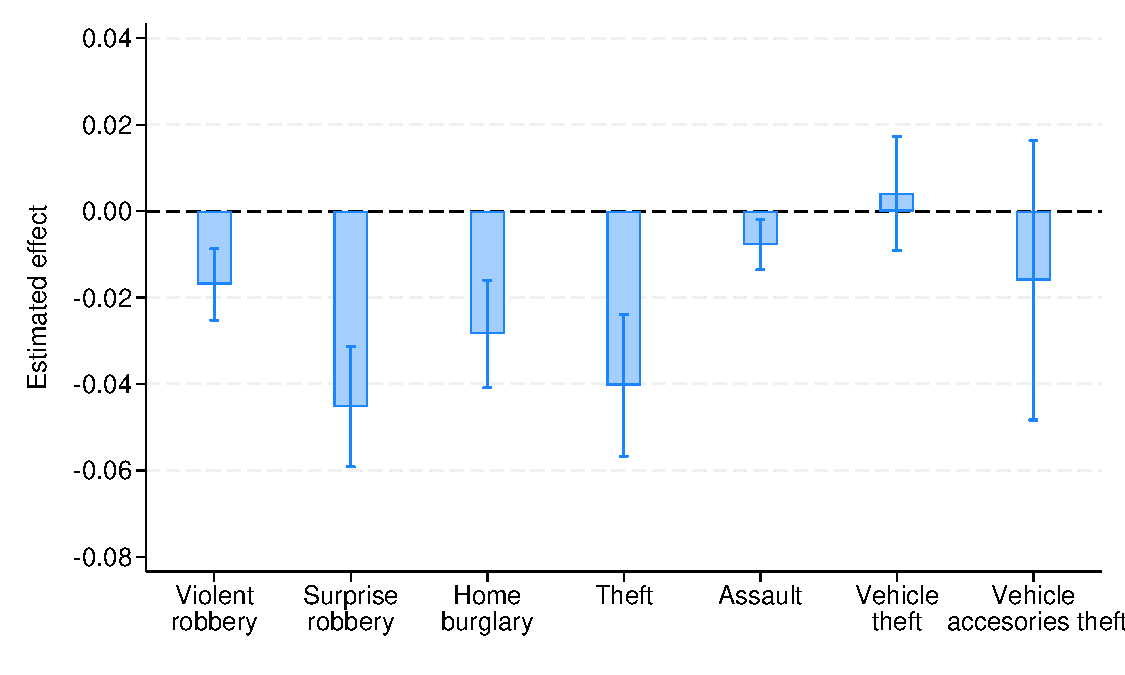
\includegraphics[width=\textwidth]{../manuscript/Graphs/results_typeofcrimes_ENUSC.pdf}
                \caption{Effects on Victimization \\ by Type of Crime}
    \end{subfigure}
    \begin{subfigure}{0.45\textwidth}
        \centering
        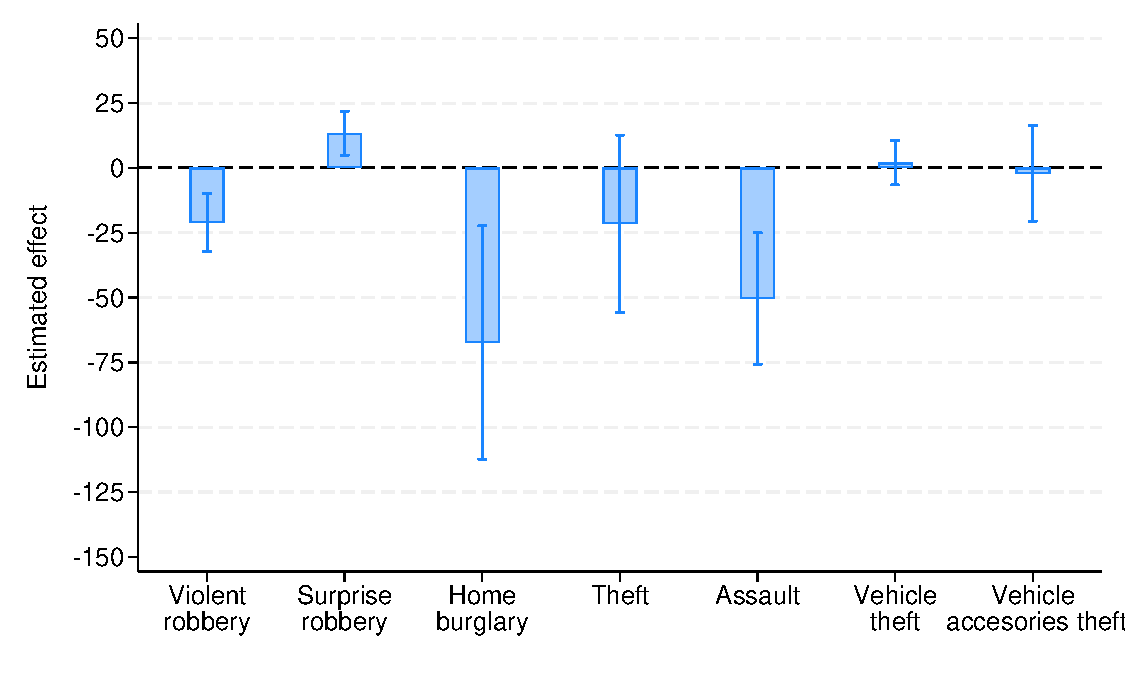
\includegraphics[width=\textwidth]{../manuscript/Graphs/results_typeofcrimes_SPD.pdf}
                \caption{Effects on Reported crime  \\ by Type of Crime}
    \end{subfigure}
    \\[12pt]
    \begin{minipage}{0.99\textwidth}
    \footnotesize Notes: This figure shows the pooled effects of the \emph{Plan Cuadrante} on victimization and number of crimes reported to the police per 100,000 inhabitants by type of crime. The estimation is conducted using the procedure developed in \citet{Callaway} for difference-in-differences with staggered treatment adoption. The graphs display the estimated coefficients and 95\% confidence intervals. Standard errors are clustered at the municipality level using the wild bootstrapping procedure.
    Panel (a) presents the results using victimization data from ENUSC surveys while Panel (b) presents the results using municipality-level administrative data on crime reported to the police provided by the Undersecretary for Crime Prevention. 
    \end{minipage}
\end{figure}
\clearpage

\subsection{Effects of \emph{Plan Cuadrante} on Crime Preventing Measures by Type of Measure and Household SES}
Table \ref{tab:hhprotectionmeasurestype} presents the effect of \emph{Plan Cuadrante} on different types of crime prevention measures by the socioeconomic status of households. The results indicate that \emph{Plan Cuadrante} reduces household investments in crime prevention measures across all socioeconomic groups, particularly investments in more affordable measures such as grilles and dogs.

\begin{table}[h!]
\caption{Effects of \emph{Plan Cuadrante} on Household Security Measures, by Type of Measure and Socioeconomic Status}
\label{tab:hhprotectionmeasurestype}
\begin{center}
\resizebox{\textwidth}{!}{
\begin{tabular}{lcccccc} \hline \hline
& (1) & (2) & (3) & (4) & (5) & (6) \\
& \multicolumn{3}{c}{Cheap measures} & \multicolumn{3}{c}{Expensive measures} \\
\cmidrule(lr){2-4} \cmidrule(lr){5-7}
& All & Higher SES & Lower SES & All & Higher SES & Lower SES \\
\cmidrule(lr){2-4} \cmidrule(lr){5-7}
\\
ATT & -0.072*** & -0.090*** & -0.058*** & -0.015*** & -0.028*** & -0.004 \\
& (0.015) & (0.018) & (0.018) & (0.005) & (0.010) & (0.005) \\
\\
N & 93,041 & 40,377 & 52,664 & 93,041 & 40,377 & 52,664 \\
Municipalities & 47 & 47 & 47 & 47 & 47 & 47 \\
Y mean & 0.176 & 0.211 & 0.151 & 0.050 & 0.085 & 0.026 \\
\hline \hline
\end{tabular}}
\par{
\begin{tabular}{p{\textwidth}}
\footnotesize{Note: This table reports the effect of \emph{Plan Cuadrante} on the probability that a household adopted a given type of security measure in the previous 12 months, using ENUSC survey data. Cheap measures are window grilles and guard dogs; expensive measures are firearms, alarms, private security insurance, and private guards. Columns (1)--(3) report the effects on cheap measures and columns (4)--(6) on expensive measures, for all households and split by household socioeconomic status (SES), with Higher SES denoting the upper SES strata and Lower SES the lower strata. The reported ATT is the average post-treatment effect, estimated with the staggered difference-in-differences procedure of \citet{Callaway}. Standard errors, clustered at the municipality level using the wild bootstrap, are reported in parentheses. The Y mean row reports the mean of the outcome among treated municipalities before adoption. ***p$<$0.01, **p$<$0.05, *p$<$0.1.} \\
\end{tabular}}
\end{center}
\end{table}

\clearpage

\subsection{Effects of \emph{Plan Cuadrante} and Changes in Police Resources}
\label{resources_plan_cuadrante} 

To make the implementation of \emph{Plan Cuadrante} possible, police resources were augmented in some municipalities. To examine the extent to which the observed results might be driven by the increase in police resources rather than by the geographic specialization component of the reform, we conduct the following two empirical exercises.

Firstly, we examine the heterogeneity of \emph{Plan Cuadrante}'s effects by the magnitude of resource increases in each municipality. Panels (a) and (b) of Figure \ref{fig:figure_resources} show that municipalities in the bottom 40\% of the resource-increase distribution---represented by blue bars---experienced increases close to the average annual variation experienced by never treated or municipalities that had not yet adopted the program (green bar), while municipalities in the top 40\% (red bars) experienced larger increases, with officers rising by around 22\% and patrol vehicles by around 80\%. If the effects of \emph{Plan Cuadrante} were driven by resource increases alone, we would not expect to see any effect in municipalities with increases in police resources similar in magnitude to those observed in the control group. To conduct our heterogeneity analysis, we split the sample into municipalities with small and large resource increases and estimate specification (\ref{eq:main}) separately for each subsample. Yet panels (c) and (d) of Figure \ref{fig:figure_resources} show that the effects on most outcomes remain sizeable for most crime and crime perception outcomes even among municipalities with resource increases similar to the control group. While there might be a resource gradient for the effects on crime perception, the effects on twelve-month victimization and private investment in security, in municipalities with resource increases similar to those in the control group, are comparable in magnitude to the effects among municipalities with larger resource increases. The effect on the probability of complaining about police surveillance, arguably a proxy for police presence, was also similar for both groups.\footnote{We provide the heterogeneous effects of \emph{Plan Cuadrante} on complaints about lack of police surveillance because information on this variable is available for the period 2003-2012. However, information on the share of households perceiving an increase in police presence, reporting that police passed by their house daily and never seeing police patrols near their house is only available in ENUSC rounds 2003, 2005 and 2006, and therefore there is not sufficient overlap with information on resources, available from 2005 for patrol vehicles and from 2006 for police officers.} More generally, we cannot reject the hypothesis that effects are equal between the two groups in all the examined outcomes. The heterogeneous effects on trust in the police, complaints about the lack of police officers, and arrests---the three outcomes not shown in Figure \ref{fig:figure_resources}---are reported in Figure \ref{fig:heterogeneity_appendix} and are likewise similar across the two groups.

\FloatBarrier
\begin{figure}[h!]
    \centering
    \caption{Effects of \emph{Plan Cuadrante} by Resource Increase: Trust, Complaints, and Arrests}
    \label{fig:heterogeneity_appendix}
    \begin{subfigure}[t]{0.48\textwidth}
        \centering
        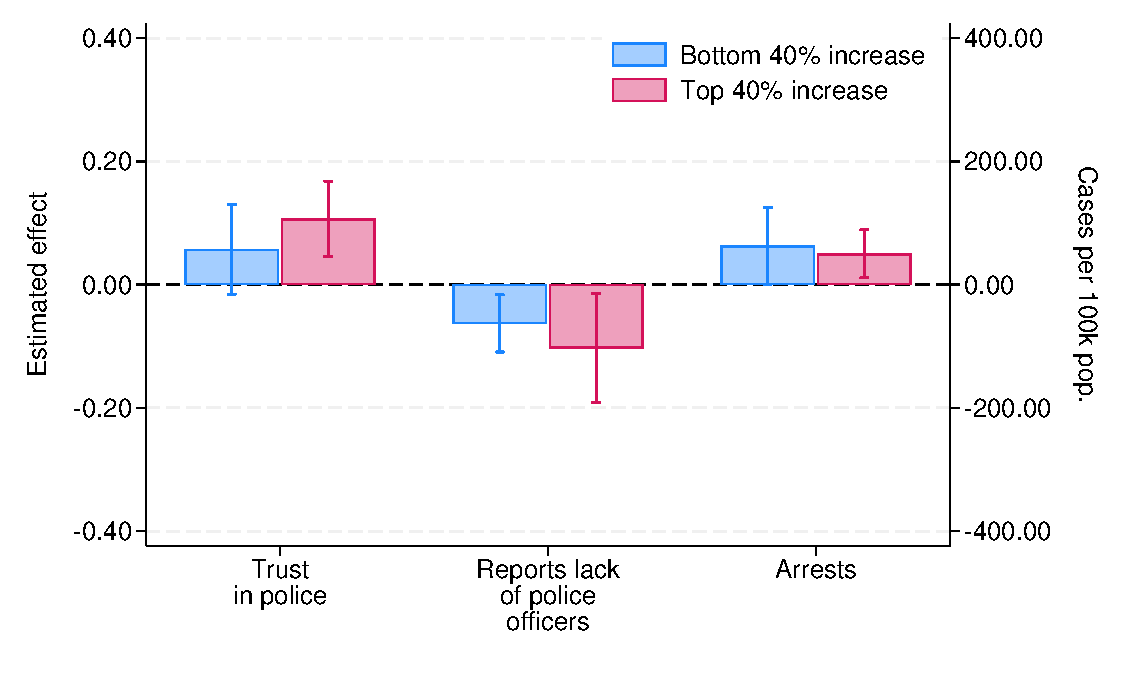
\includegraphics[width=\linewidth]{../manuscript/Graphs/heterogeneity_off_appendix.pdf}
        \caption{By the intensity of $\Delta$ in police officers}
    \end{subfigure}\hfill
    \begin{subfigure}[t]{0.48\textwidth}
        \centering
        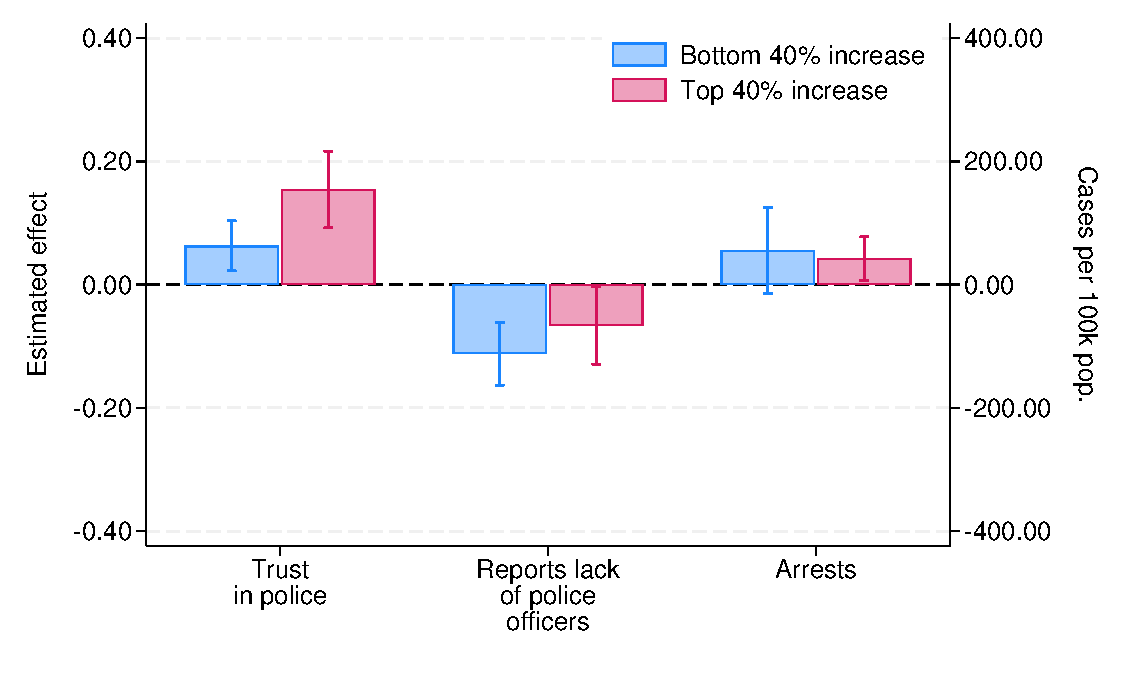
\includegraphics[width=\linewidth]{../manuscript/Graphs/heterogeneity_pv_appendix.pdf}
        \caption{By the intensity of $\Delta$ in patrol vehicles}
    \end{subfigure}
    \\[8pt]
    \begin{minipage}{0.99\textwidth}
    \footnotesize Notes: This figure complements Figure \ref{fig:figure_resources} by reporting, for the three outcomes not shown there, the effect of \emph{Plan Cuadrante} estimated separately for municipalities in the bottom 40\% (blue) and top 40\% (red) of the resource-increase distribution. Panel (a) splits municipalities by the increase in police officers and panel (b) by the increase in patrol vehicles. In each panel, arrests (administrative data, in cases per 100,000 inhabitants) are read on the right axis; the other two outcomes, from the ENUSC survey (trust in the police, and reports about the lack of police officers), are read on the left axis. Effects are estimated using the difference-in-differences estimator for staggered treatment adoption developed in \citet{Callaway}; bars are point estimates and whiskers 95\% confidence intervals, with standard errors clustered at the municipality level using the wild bootstrapping procedure.
    \end{minipage}
\end{figure}

\FloatBarrier

Finally, we re-estimate the main results of the study reported in Figure \ref{fig:figure02}, controlling for the number of police officers and the number of patrol vehicles in the municipality.

The results of this analysis are reported in Table \ref{tab:results_controlbyresources}. The magnitude of the estimated effects remains similar for most variables, although the statistical significance is reduced in some estimations. This likely reflects a mechanical feature of the \citet{Callaway} estimation procedure: control variables are not incorporated parametrically, but are instead used to construct the comparison group via outcome regression or propensity-score weighting, so the resulting estimation uncertainty propagates to the ATT standard errors. Note, however, that these resource variables are bad controls, as they are affected by the adoption of \emph{Plan Cuadrante}, so these results should be interpreted with caution.


\begin{table}[h!]\centering
\caption{Effects of \emph{Plan Cuadrante} Controlling for Police Resources}
\label{tab:results_controlbyresources}
\resizebox{\textwidth}{!}{
\begin{threeparttable}
\begin{tabular}{l ccccc}
\toprule
 & (1) & (2) & (3) & (4) & (5) \\
\midrule
\multicolumn{6}{l}{\textit{Panel A. Victimization}} \\[0.2em]
ATT &       -0.099*** &       -0.077*** &       -0.086** &       -0.094*** &       -0.087* \\
  & (0.013) & (0.013) & (0.043) & (0.028) & (0.053) \\
N &    93,041 &    53,973 &    53,553 &    72,017 &    53,553 \\[0.4em]
\multicolumn{6}{l}{\textit{Panel B. Crime perception}} \\[0.2em]
ATT &       -0.149*** &       -0.140*** &       -0.112** &       -0.082** &       -0.111 \\
  & (0.025) & (0.032) & (0.057) & (0.033) & (0.106) \\
N &    89,578 &    52,160 &    51,746 &    69,434 &    51,746 \\[0.4em]
\multicolumn{6}{l}{\textit{Panel C. Investment in security measures}} \\[0.2em]
ATT &       -0.077*** &       -0.066*** &       -0.109*** &       -0.081*** &       -0.168*** \\
  & (0.016) & (0.019) & (0.041) & (0.019) & (0.064) \\
N &    93,041 &    53,973 &    53,553 &    72,017 &    53,553 \\[0.4em]
\multicolumn{6}{l}{\textit{Panel D. Reported crime (per 100k pop.)}} \\[0.2em]
ATT &     -208.024*** &     -190.446*** &       29.230 &     -261.439 &     -245.555 \\
  & (56.130) & (67.908) & (147.261) & (170.954) & (165.221) \\
N &     4,231 &     1,918 &     1,911 &     2,248 &     1,911 \\[0.4em]
\midrule
Sample                   & Full & Resource yrs & Resource yrs & Resource yrs & Resource yrs \\
Police officers (per 100k pop.) &      &            & \checkmark &            & \checkmark \\
Patrol vehicles (per 100k pop.) &      &            &            & \checkmark & \checkmark \\
\bottomrule
\end{tabular}
\begin{tablenotes}[flushleft]
\item \footnotesize{Note: ATT estimates of the effect of \emph{Plan Cuadrante} on each outcome. Column (1) is the baseline (full estimation sample, no controls) and reproduces the headline estimate of the corresponding estimator. Column (2) restricts the estimation to 2006--2012, the window over which police resources are observed, without including any control variable. Columns (3)--(5) add time-varying controls for police resources per 100{,}000 inhabitants: officers only; patrol vehicles only; and officers and patrol vehicles jointly (entered as separate regressors). Columns (3) and (5) cover 2006--2012, the years for which the number of officers is observed; column (4) also includes 2005, the first year for which patrol vehicles are observed. Patrol vehicles are measured, per 100{,}000 inhabitants, as all patrol automobiles (radiopatrulla, auto patrullero, auto policial, automovil, station wagon, jeep and camioneta) plus motorcycles. Standard errors in parentheses; row N reports the estimation-sample size. Estimation follows \citet{Callaway}; standard errors clustered at the municipality level using wild bootstrapping procedures. $^{*}p<0.1$, $^{**}p<0.05$, $^{***}p<0.01$.}
\end{tablenotes}
\end{threeparttable}}
\end{table}


\clearpage

\subsection{Factors Associated with the Increase in Police Resources}
\label{sec:resource_correlates}

As discussed in Section \ref{institutions} and in Online Appendix \ref{resources_plan_cuadrante}, the increase in police resources associated with the adoption of \emph{Plan Cuadrante} varied substantially across municipalities. In principle, this increase should be related to each municipality's pre-existing police resource deficit---measured in Equivalent Surveillance Units (UVEs)---which \emph{Plan Cuadrante} was meant to help close. However, program evaluations do not clearly establish that this deficit is what determined the size of the resource increase each municipality received \citep{DIPRES2007_largo,DIPRES2014}.\footnote{Although we requested information on the demand and supply of UVEs underlying this allocation, this information was not provided by \textit{Carabineros}.} If the pre-existing deficit is not what determines the resource increase, what is it related to? Reassuringly, municipalities receiving larger versus smaller resource increases do not display differential pre-treatment trends in either the outcomes of interest or in police resources themselves.\footnote{We test for the joint significance of the pre-treatment coefficients between the two groups, separately for the split based on the increase in police officers and the split based on the increase in patrol vehicles. The resulting p-values are, respectively, 0.823 and 0.048 for victimization, 0.059 and 0.379 for crime perception, 0.820 and 0.157 for investment in security measures, and 0.213 and 0.419 for reported crime, as well as 0.616 and 0.444 for police officers and 0.405 and 0.157 for patrol vehicles.} In this section we examine whether the magnitude of the resource increase experienced by a municipality upon adoption is correlated with its pre-treatment levels in crime, police resources, and other observable characteristics. Specifically, we regress the increase in resources at the time of adopting \emph{Plan Cuadrante} on municipality characteristics measured before the program's introduction, including crime and police resources in 2006, the first year for which information on police resources is available. Thus, we restrict this analysis to municipalities that adopted \emph{Plan Cuadrante} from 2007 onward.

Table \ref{tab:resourcecorrelates} reports OLS regressions of the average annual increase in police officers and patrol vehicles per 100,000 inhabitants on pre-adoption municipality characteristics, separately for the administrative (SPD) sample at the municipality level (columns 1--2) and the ENUSC sample at the survey-respondent level (columns 3--4). All variables are standardized and standard errors are clustered by municipality, so coefficients are comparable in magnitude across regressors.

The results provide little support for the hypothesis that municipalities with worse pre-treatment crime outcomes received systematically larger resource increases. Pre-treatment reported crime is, if anything, negatively associated with the subsequent increase in both officers and vehicles in the administrative sample (columns 1--2); in the ENUSC sample, it is negatively associated with the increase in officers (column 3), although it is positively associated with the increase in vehicles (column 4). Pre-treatment victimization is, if anything, negatively associated with both increases in the ENUSC sample (columns 3--4). Pre-treatment arrests, crime perception, trust in the police, and private investment in security measures are not significantly associated with the resource increase. The increase in resources is instead more strongly predicted by structural municipality characteristics: less populous municipalities experienced larger increases in three of the four specifications, and municipalities with higher poverty rates predicted a larger increase in vehicles in the administrative sample (column 2), although this association is not significant for officers in that sample (column 1) or in the ENUSC sample (columns 3--4).

\begin{table}[H]
\centering
\caption{Predictors of the Increase in Police Resources under \emph{Plan Cuadrante}}
\label{tab:resourcecorrelates}
\begin{threeparttable}
\small
\setlength{\tabcolsep}{6pt}
\renewcommand{\arraystretch}{1.1}
\begin{tabular}{@{}l cc cc@{}}
\toprule
& \multicolumn{2}{c}{Administrative sample} & \multicolumn{2}{c}{ENUSC sample} \\
\cmidrule(lr){2-3} \cmidrule(lr){4-5}
& Police & Patrol & Police & Patrol \\
Dep.\ var: avg.\ annual increase & officers & vehicles & officers & vehicles \\
in resources (share of pre-adoption level) & (1) & (2) & (3) & (4) \\
\midrule
Reported crime (per 100k pop.) & $-0.203^{**}$ & $-0.199^{**}$ & $-0.319^{*}$ & $0.272^{*}$ \\
 & (0.099) & (0.097) & (0.182) & (0.137) \\
Arrests (per 100k pop.) & $0.099$ & $-0.041$ & $0.003$ & $0.297$ \\
 & (0.136) & (0.129) & (0.186) & (0.223) \\
Victimization &  &  & $-0.017^{*}$ & $-0.025^{*}$ \\
 &  &  & (0.010) & (0.013) \\
Crime perception &  &  & $0.005$ & $0.008$ \\
 &  &  & (0.017) & (0.014) \\
Trust in the police &  &  & $0.024$ & $0.027$ \\
 &  &  & (0.018) & (0.019) \\
Investment in security measures &  &  & $0.004$ & $-0.003$ \\
 &  &  & (0.010) & (0.009) \\
Police officers (per 100k pop.) & $-0.207$ & $0.155$ & $-0.888^{***}$ & $0.571^{***}$ \\
 & (0.155) & (0.129) & (0.154) & (0.136) \\
Patrol vehicles (per 100k pop.) & $-0.129$ & $-0.139$ & $0.537^{**}$ & $-0.507^{***}$ \\
 & (0.129) & (0.126) & (0.212) & (0.169) \\
Log population & $-0.529^{***}$ & $-0.203^{*}$ & $-0.193$ & $-0.626^{**}$ \\
 & (0.145) & (0.112) & (0.189) & (0.269) \\
Poverty rate (2004) & $0.170$ & $0.308^{**}$ & $0.027$ & $-0.017$ \\
 & (0.113) & (0.126) & (0.108) & (0.108) \\
\midrule
Observations & 65 & 65 & 8,781 & 8,781 \\
R-squared & 0.342 & 0.282 & 0.614 & 0.545 \\
\bottomrule
\end{tabular}
\begin{tablenotes}[flushleft]
\footnotesize
\item \textit{Note:} OLS regressions of the average annual increase in police officers (columns 1 and 3) and patrol vehicles (columns 2 and 4) per 100{,}000 inhabitants, from the year before adoption of \emph{Plan Cuadrante} to 2012. As in panels (a) and (b) of Figure \ref{fig:figure_resources}, the increase is expressed as a share of the resources available the year before adoption. Columns 1--2 use the administrative sample at the municipality level; columns 3--4 use ENUSC survey respondents interviewed before 2007 (survey outcomes at the respondent level, other regressors as pre-2006 municipality aggregates). All variables are standardized. Standard errors clustered by municipality in parentheses.
\item $^{*}p<0.1$; $^{**}p<0.05$; $^{***}p<0.01$.
\end{tablenotes}
\end{threeparttable}
\end{table}


\clearpage

\subsection{Police Resources and Police Effectiveness}
\label{resources_vs_specialization}

This Online Appendix presents two additional empirical analyses examining the link between police resources and crime in Chile, outside the scope of \emph{Plan Cuadrante}.

First, we assess the effects of \textit{Seguridad Ciudadana}, a program that creates a security force that, while they do not have the competence to apprehend or carry weapons, assist Carabineros in their work, effectively increasing their human resources for tasks such as patrolling and other deterrence activities. Like \emph{Plan Cuadrante}, the creation of these municipal security forces was staggered and started after 2012 in nearly all municipalities.\footnote{Among the municipalities in the ENUSC survey, only Curic\'o introduced the \textit{Seguridad Ciudadana} program before 2013, being 2012 the last year in which \emph{Plan Cuadrante} was implemented for the first time in a municipality surveyed in ENUSC. Among the full set of 346 municipalities, only 10 of them introduced the program \textit{Seguridad Ciudadana} before 2013, all of them except Curic\'o being small municipalities.} We hand-collected the year in which each municipality established its \textit{Seguridad Ciudadana} program, requesting this information from all 346 Chilean municipalities through the national transparency portal (\emph{Portal de Transparencia}) and compiling the responses they returned into an original dataset. Using administrative and ENUSC data available until 2017, the estimated effects of \textit{Seguridad Ciudadana} program are presented in Figure \ref{fig:figureA5}. We estimate the effects for all the outcomes examined in the \emph{Plan Cuadrante} analysis except for trust in the police, since information on the latter variable is rarely collected in ENUSC rounds conducted after 2012. The results show that this program had little effects on every dimension of police effectiveness considered. This result is also consistent with the hypothesis that the large effects of \emph{Plan Cuadrante} on police effectiveness are unlikely driven entirely by the change in police resources brought by the program.

\begin{figure}[h!]
    \centering
    \caption{Effects of \textit{Seguridad Ciudadana} on Crime Outcomes and Security Perceptions}
    \label{fig:figureA5}
    
    % Primera fila: panel (a) y (b)
    \begin{subfigure}{0.495\textwidth}
        \centering
        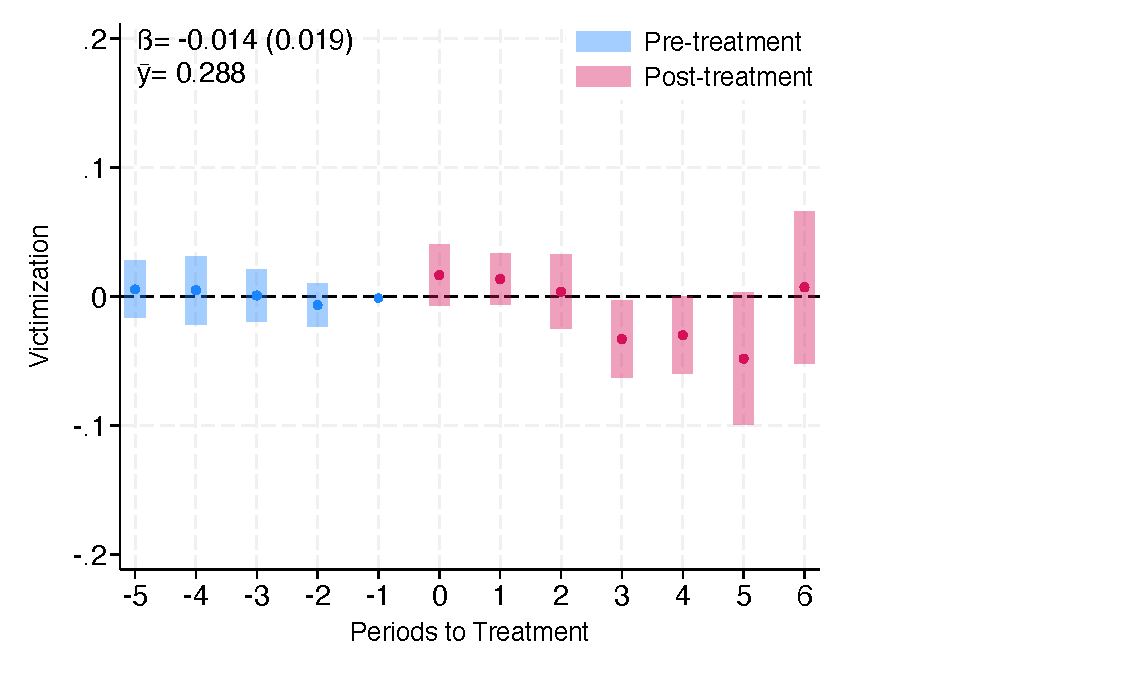
\includegraphics[width=\textwidth]{../manuscript/Graphs/results_victimization_SC.pdf}
        \caption{Victimization in last 12 months}
    \end{subfigure}%
    \hfill
    \begin{subfigure}{0.495\textwidth}
        \centering
        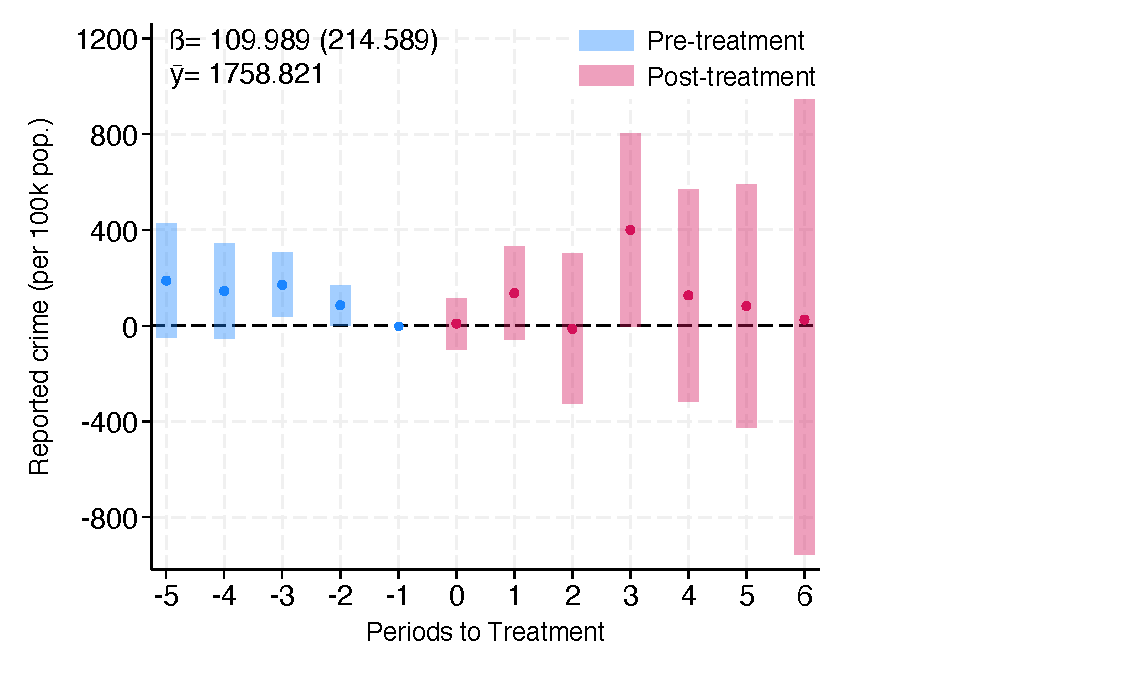
\includegraphics[width=\textwidth]{../manuscript/Graphs/totalreportedcrime_allcomunas_SC.pdf}
        \caption{Reported crime per 100k inhabitants}
    \end{subfigure}

    \vspace{12pt} % Espacio entre filas
    
    % Segunda fila: panel (c) y (d)
    \begin{subfigure}{0.495\textwidth}
        \centering
        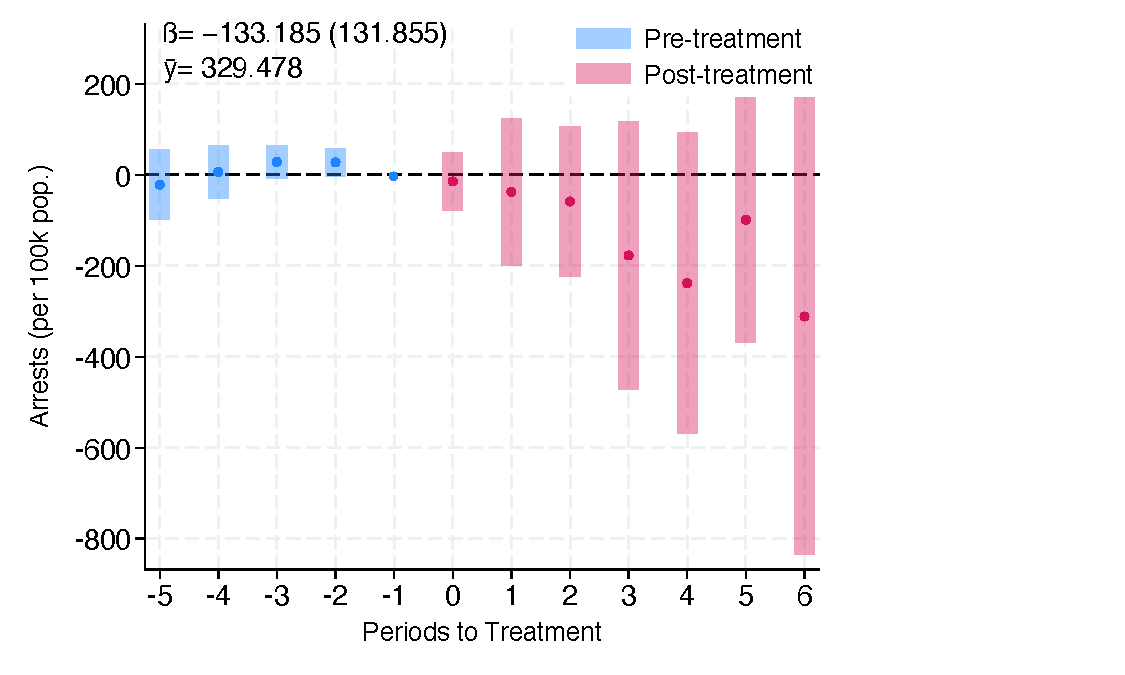
\includegraphics[width=\textwidth]{../manuscript/Graphs/totalarrestscrime_allcomunas_SC.pdf}
        \caption{Arrests per 100k inhabitants}
    \end{subfigure}%
    \hfill
    \begin{subfigure}{0.495\textwidth}
        \centering
        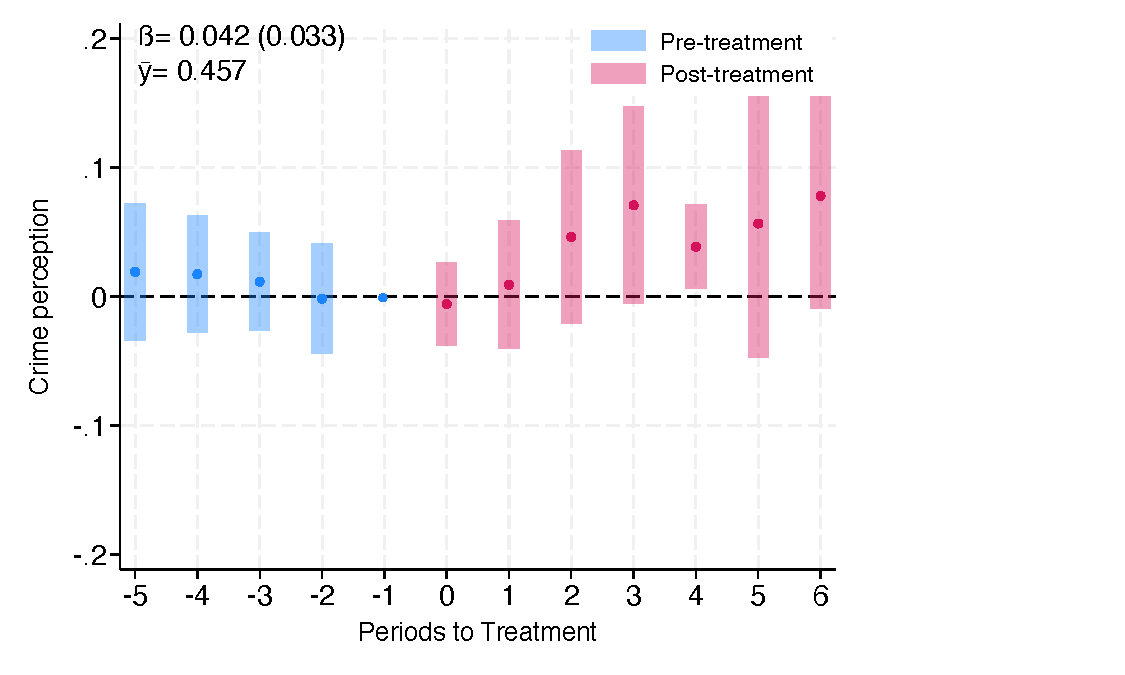
\includegraphics[width=\textwidth]{../manuscript/Graphs/results_perception_SC.pdf}
        \caption{Households reporting an \\ increase in crime}
    \end{subfigure}
    
    \vspace{12pt} % Espacio entre filas
    
    % Tercera fila: panel (e)
    \begin{subfigure}{0.495\textwidth}
        \centering
        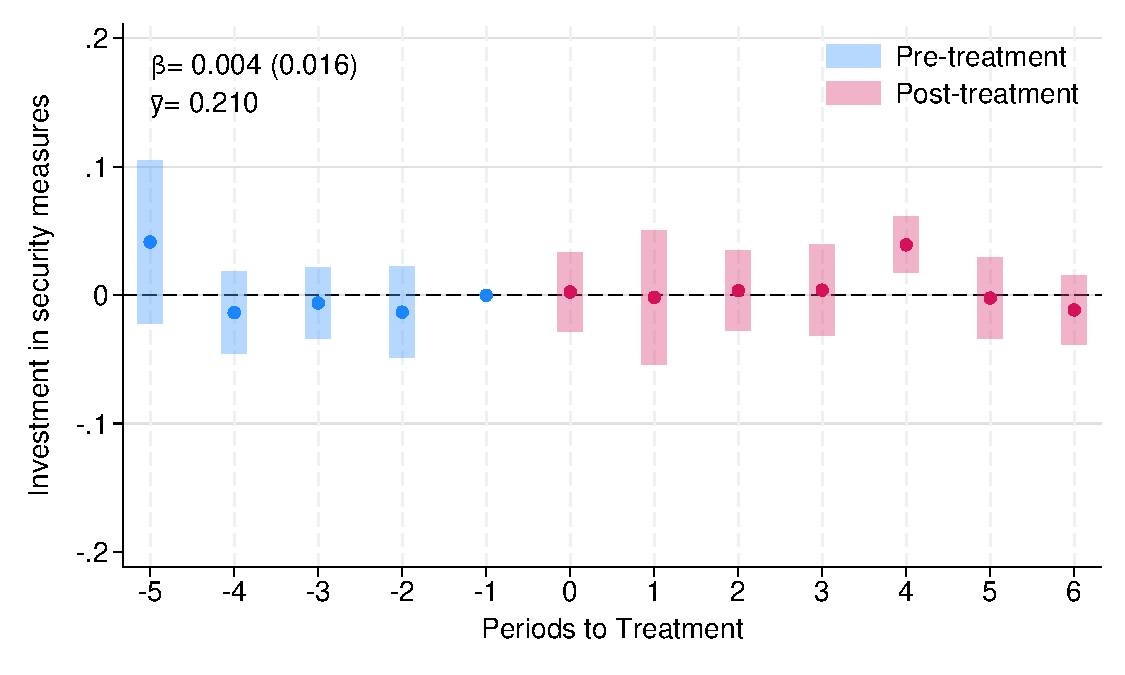
\includegraphics[width=\textwidth]{../manuscript/Graphs/results_hhprotectionmeasures_SC.pdf}
        \caption{Households adopting security measures}
    \end{subfigure}

    \vspace{12pt} % Espacio para las notas
    
    \begin{minipage}{0.99\textwidth}
        \footnotesize
        Notes: This figure shows the dynamic effects of the \textit{Seguridad Ciudadana} program on different measures of crime and security perceptions. The estimation is conducted using the procedure developed in \citet{Callaway} for difference-in-differences with staggered treatment adoption. The dots in the figure represent the estimated coefficients and the bars behind them 95\% confidence intervals. Standard errors are clustered at the municipality level using wild bootstrapping. The pooled effect and the mean outcome before the introduction of the treatment for the outcome---computed as in Figure \ref{fig:figure02}, using only the pre-treatment observations of treated units---is also presented in each panel. Panel (a) reports the effect of \textit{Seguridad Ciudadana} on the probability of household victimization in the last 12 months using the ENUSC survey. Panel (b) reports the effect on the number of crimes reported to the police in the municipality per 100,000 inhabitants using administrative data. Panel (c) reports the effect on the number of arrests in the municipality per 100,000 inhabitants using administrative data. Panel (d) reports the effect on the probability of perceiving an increase in crime using the ENUSC survey. Panel (e) reports the effect on the probability of adopting security measures in the last twelve months using the ENUSC survey. Panel (a) includes 210,102 observations; panel (b), 2,234; panel (c), 1,908; panel (d), 203,078; and panel (e), 74,316 observations.
    \end{minipage}
\end{figure}

\clearpage

Secondly, we use yearly information on the number of police officers and patrol vehicles at the municipality level facilitated by \textit{Carabineros} for the period 2006-2012 to examine the statistical association between police resources and crime, controlling for year and municipality fixed effects. Specifically, we estimate the following regression:

\begin{equation}
Crime_{imt}=  \delta_{1} \mbox{\textit{Police resources}}_{mt} +  Municipality_{m}   +      Year_{t} +  u_{imt}
\label{eq:correlation}
\end{equation}

\noindent where \textit{Police resources} indicates either the number of police officers per 100,000 inhabitants in municipality $m$ during year $t$ or the number of patrol vehicles per 100,000 inhabitants in municipality $m$ during year $t$. We focus on the 41 municipalities of Santiago surveyed in ENUSC for the period 2006-2012. The study period is delimited by the availability of data on police resources. We focus on the municipalities of Santiago because \emph{Plan Cuadrante} was implemented in all of these municipalities by 2000. Expanding the analysis to other municipalities may confound the dynamic effects of \emph{Plan Cuadrante} with the potential effects of subsequent increases in police resources. Between 2006 and 2012, these municipalities saw an average increase of 26\% in police officers and 83\% in patrol vehicles.

The results of the analyses are reported in Figure \ref{fig:figureA7B}. While the set of fixed effects account for time-invariant unobservable characteristics of the municipalities and the time shocks that affects all municipalities at the same time, the coefficients should be interpreted with caution due to potential endogeneity concerns. Overall, the results show little statistical association between police resources and the different outcomes examined, except for perceived crime. The lack of statistical association between police resources and the main outcomes is consistent with the increase of resources playing a limited role in explaining the effects of \emph{Plan Cuadrante}. Figure \ref{fig:figureA7B} reports these associations for two samples shown side by side: the 41 metropolitan municipalities of Santiago (blue bars) and the broader set of municipalities that implemented \emph{Plan Cuadrante} before 2006 together with the never treated municipalities surveyed in ENUSC (red bars). The results are similar across both samples.

\begin{figure}[h!]
    \centering
    \caption{Association between Police Resources and Police Effectiveness (No \emph{Plan Cuadrante} Variation)}
    \label{fig:figureA7B}
    \begin{subfigure}[t]{0.48\textwidth}
        \centering
        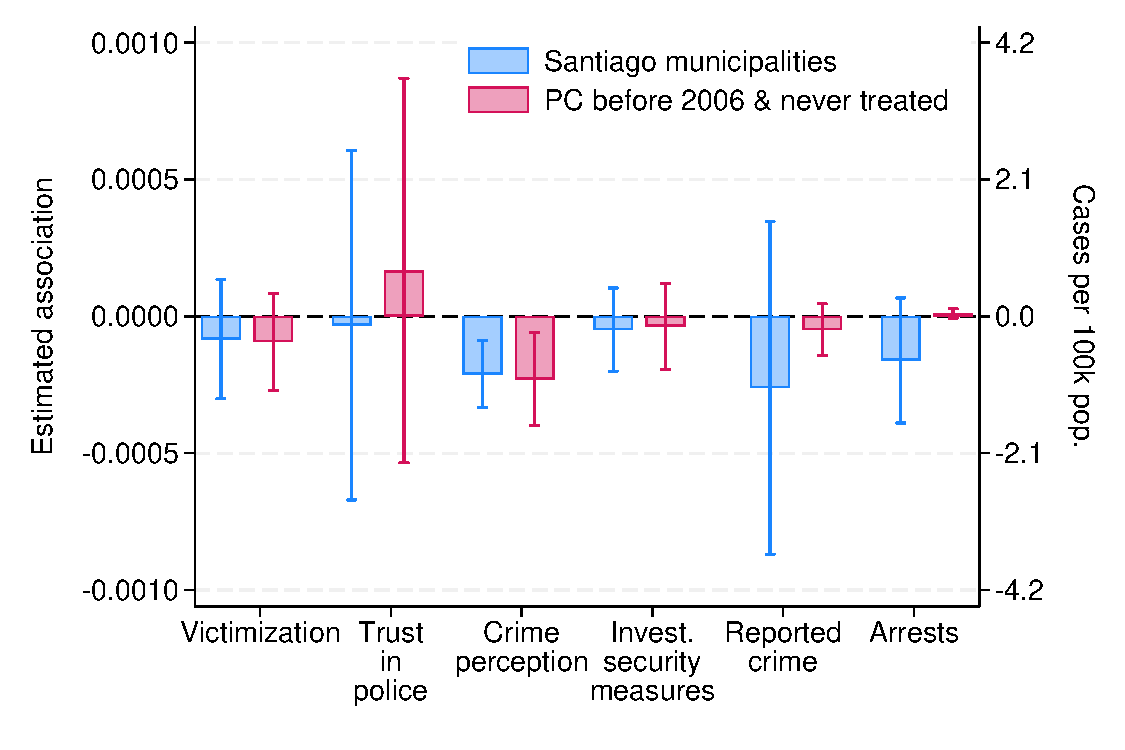
\includegraphics[width=\linewidth]{../manuscript/Graphs/results_corr_novariation_off.pdf}
        \caption{Association with police officers}
    \end{subfigure}\hfill
    \begin{subfigure}[t]{0.48\textwidth}
        \centering
        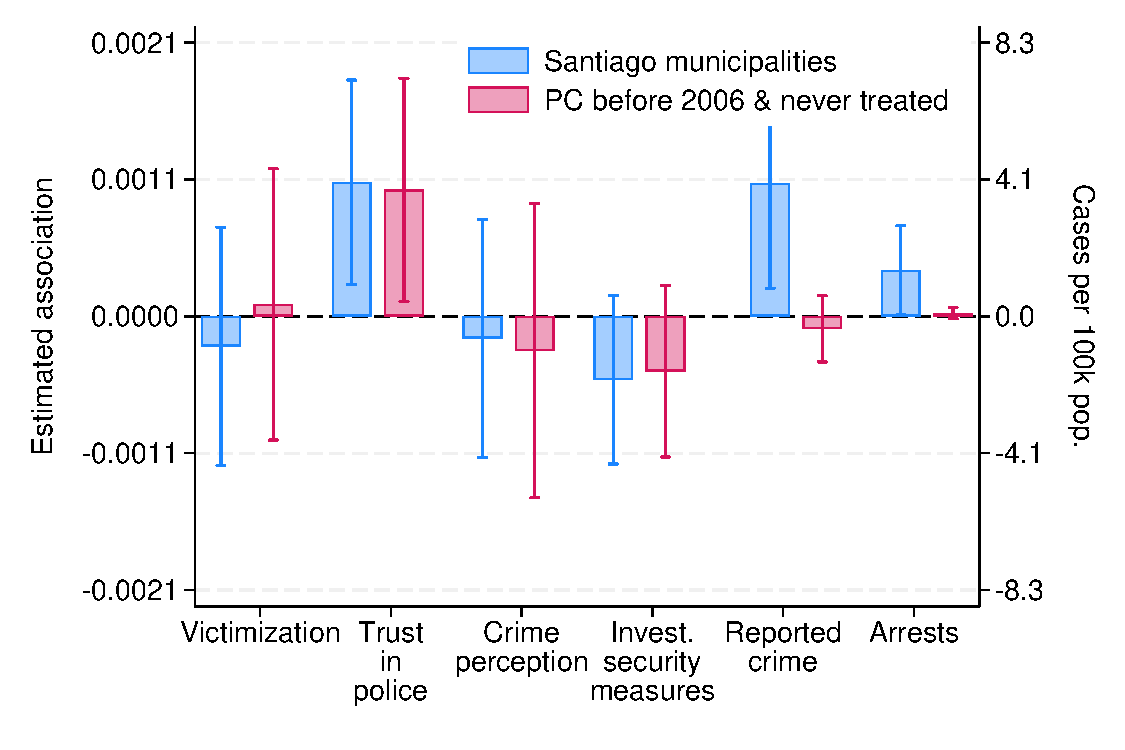
\includegraphics[width=\linewidth]{../manuscript/Graphs/results_corr_novariation_veh.pdf}
        \caption{Association with patrol vehicles}
    \end{subfigure}
    \\[10pt]
    \begin{minipage}{0.99\textwidth}
    \footnotesize Notes: The figure shows the estimated within-municipality association between police resources (per 100,000 inhabitants) and the main outcomes, in municipalities where \emph{Plan Cuadrante} does not vary over the sample period. Estimates come from OLS regressions of each outcome on the resource measure with municipality and year fixed effects; standard errors are clustered at the municipality level. Blue bars use the 41 metropolitan municipalities of Santiago, all of which adopted \emph{Plan Cuadrante} in 2000; red bars use the broader set of municipalities that adopted \emph{Plan Cuadrante} before 2006 together with the never-treated municipalities surveyed in ENUSC (2006--2012). Reported crime and arrests (administrative data, in cases per 100,000 inhabitants) are read on the right axis; all other outcomes, from the ENUSC survey (victimization, trust in the police, crime perception, and investment in security measures), are read on the left axis. Panel (a) reports associations with the number of police officers; panel (b) with the number of patrol vehicles. Bars are point estimates with 95\% confidence intervals.
    \end{minipage}
\end{figure}

\clearpage

\subsection{Adoption Timing and Perceived Police Performance}
\label{sec:balance_doseresponse}

Information on perceived police performance is only available in the 2005 round of ENUSC, so the comparison in Figure \ref{fig:figure05} relies on a single cross-section, comparing municipalities that had already adopted \emph{Plan Cuadrante} by 2005 (early adopters) with those that had not yet done so (late adopters). We consider seven measures of perceived police performance: the share of respondents who perceive police performance as good, and who perceive the police to be efficient, helpful, well informed, corrupt, failing to control crime, and failing to do their job well.


We start by assessing whether adoption timing is correlated with police performance. Using the sample of municipalities that introduced \emph{Plan Cuadrante} after 2005, Panel (a) of Figure \ref{fig:balance_doseresponse} examines the correlation between adoption timing and perceived police performance in 2005. The estimated coefficients are close to zero and statistically insignificant at conventional confidence levels, indicating that how soon a not-yet-treated municipality would go on to adopt the program is unrelated to its perceived police performance before treatment.

In Panel (b) of Figure \ref{fig:balance_doseresponse} we re-estimate the analysis conducted in Figure \ref{fig:figure05} but measuring years of exposure to \emph{Plan Cuadrante} in 2005 rather than simply whether they have adopted it or not. The results are qualitatively similar to those estimates reported in Figure \ref{fig:figure05}, showing strong correlations between years of exposure to \emph{Plan Cuadrante} and perceived police performance.

\begin{figure}[H]
    \centering
    \caption{Timing of Adoption of \emph{Plan Cuadrante} and Perceived Police Performance}
    \label{fig:balance_doseresponse}
    \begin{subfigure}{0.495\textwidth}
        \centering
        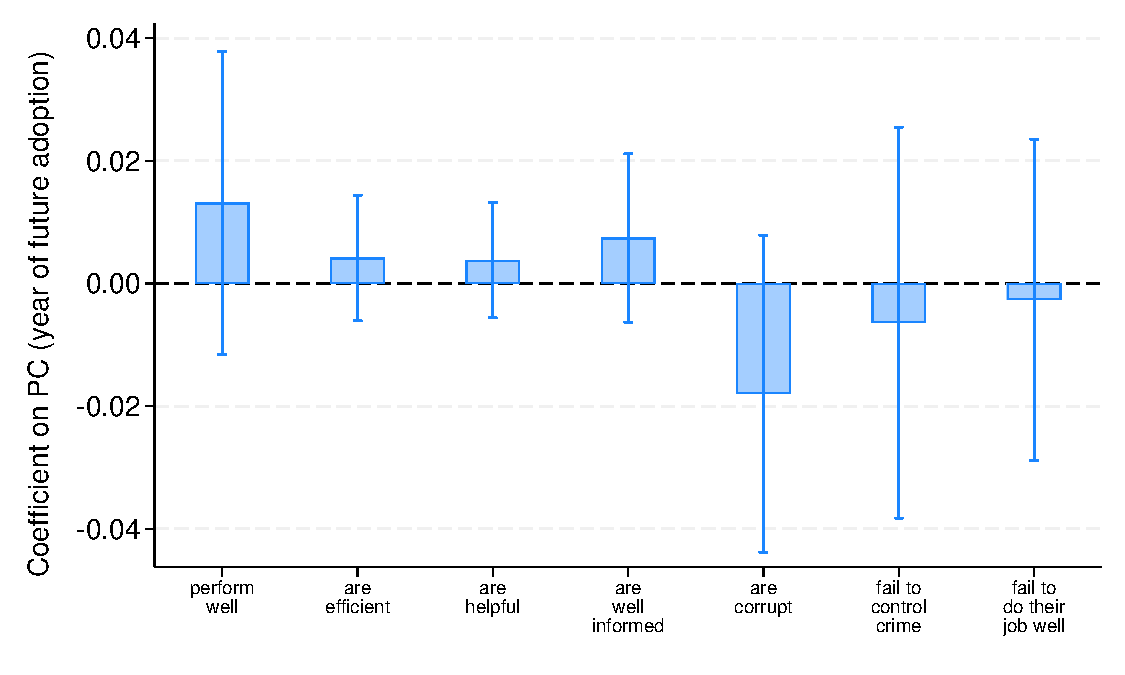
\includegraphics[width=\textwidth]{../manuscript/Graphs/balance_carabperc.pdf}
        \caption{Year of adoption and police performance before adoption}
    \end{subfigure}%
    ~
    \begin{subfigure}{0.495\textwidth}
        \centering
        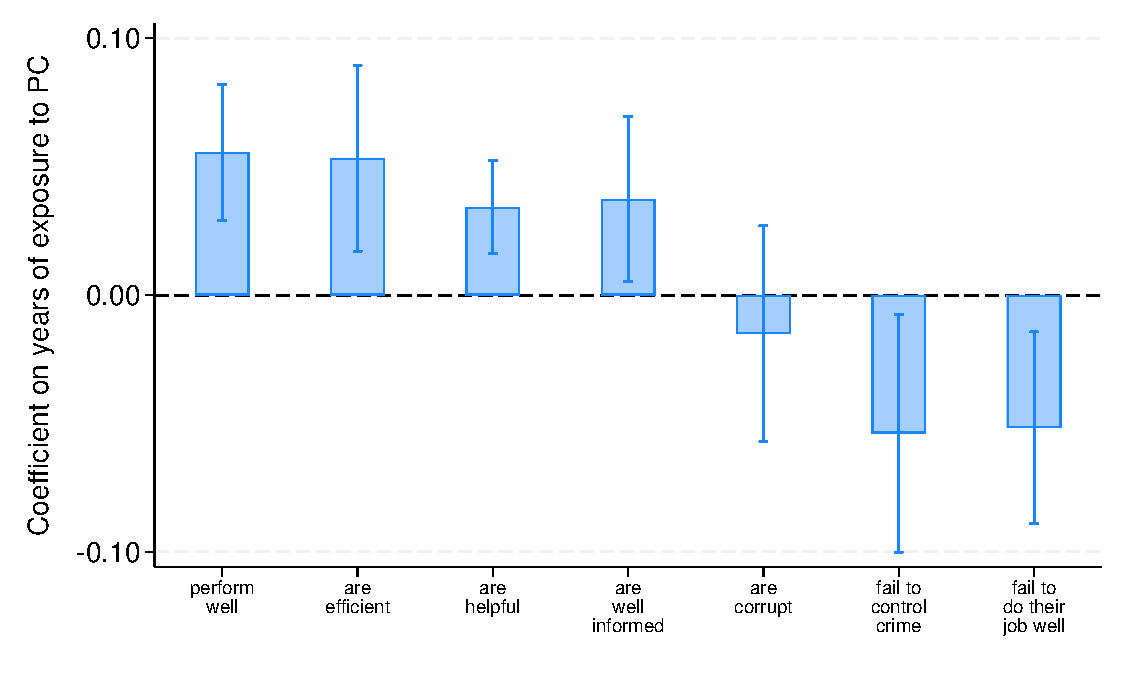
\includegraphics[width=\textwidth]{../manuscript/Graphs/doseresponse_carabperc.pdf}
        \caption{Years exposed to \emph{Plan Cuadrante} (dose response)}
    \end{subfigure}%
    \\[12pt]
    \begin{minipage}{0.99\textwidth}
    Notes: The figure considers seven measures of police performance: the share of respondents who perceive police performance as good, and who perceive the police to be efficient, helpful, well informed, corrupt, failing to control crime, and failing to do their job well. Using the sample of municipalities that adopted \emph{Plan Cuadrante} after 2005, panel (a) examines whether the future timing of adoption of \emph{Plan Cuadrante} is correlated with perceived police performance in 2005, before the introduction of the program. Panel (b) reestimates the same comparison as Figure \ref{fig:figure05}, replacing the binary adoption indicator with the municipality's number of years of exposure to \emph{Plan Cuadrante} as of 2005. In both panels, each bar plots the coefficient from a separate regression of one performance measure. The graphs display the estimated coefficients and 95\% confidence intervals.
    \end{minipage}
\end{figure}

\clearpage